\section{Backtracking}

Backtracking is a DFS-based algorithmic technique where we try all possible paths
and \textbf{backtrack} (undo choices) when we hit a dead-end.


\subsection{Q1: Determine if a valid root-to-leaf path exists}

\textbf{Q:} Determine if a path exists from the root to a leaf node such that no node in the path contains $0$.

\begin{verbatim}
boolean canReachLeaf(TreeNode root) {
    if (root == null || root.val == 0) return false;

    if (root.left == null && root.right == null)
        return true;

    if (canReachLeaf(root.left)) return true;
    if (canReachLeaf(root.right)) return true;

    return false;
}
\end{verbatim}

\textbf{Step-by-step traversal:}

\begin{center}
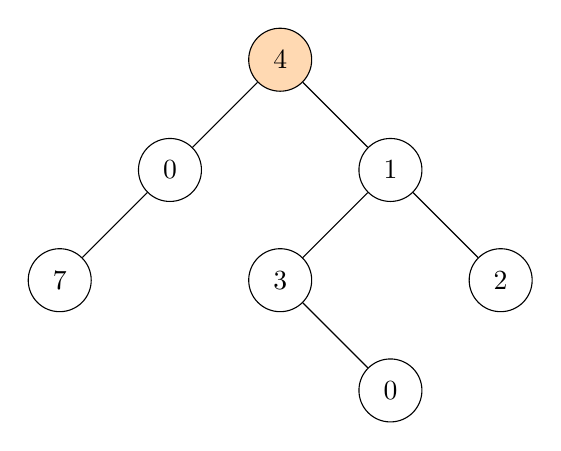
\begin{tikzpicture}[
  level distance=1.4cm,
  sibling distance=2.8cm,
  every node/.style={circle, draw, minimum size=8mm},
  edge from parent/.style={draw,-},
  curr/.style={circle, draw, fill=orange!30}
]
\node[curr] {4}
  child { node {0}
    child { node {7} }
    child[missing] {}
  }
  child { node {1}
    child { node {3}
      child[missing] {}
      child { node {0} }
    }
    child { node {2} }
  };
\end{tikzpicture}

{\small Start at root (4)}
\end{center}

\begin{center}
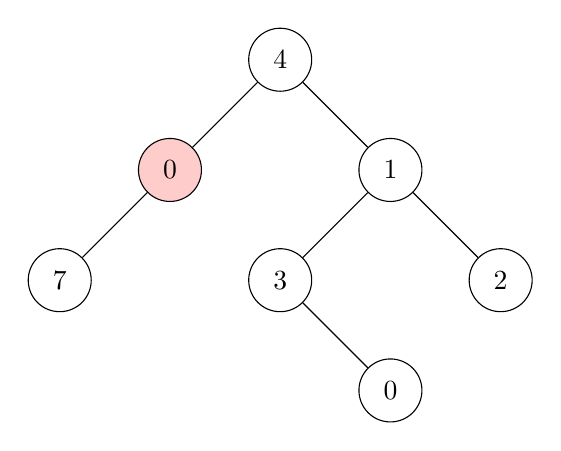
\begin{tikzpicture}[
  level distance=1.4cm,
  sibling distance=2.8cm,
  every node/.style={circle, draw, minimum size=8mm},
  edge from parent/.style={draw,-},
  bad/.style={circle, draw, fill=red!20}
]
\node {4}
  child { node[bad] {0}
    child { node {7} }
    child[missing] {}
  }
  child { node {1}
    child { node {3}
      child[missing] {}
      child { node {0} }
    }
    child { node {2} }
  };
\end{tikzpicture}

{\small Left subtree fails (contains 0), return false $\Rightarrow$ backtrack}
\end{center}

\begin{center}
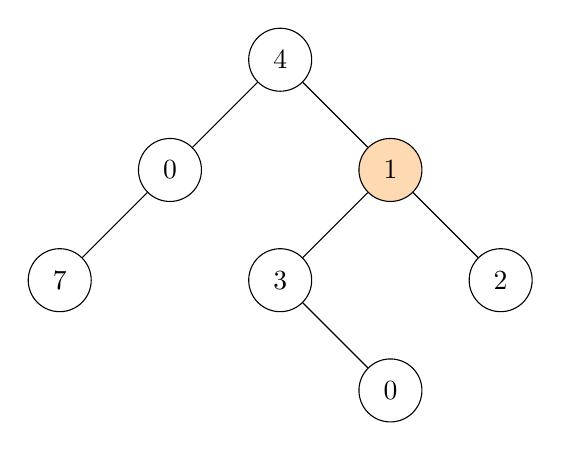
\begin{tikzpicture}[
  level distance=1.4cm,
  sibling distance=2.8cm,
  every node/.style={circle, draw, minimum size=8mm},
  edge from parent/.style={draw,-},
  curr/.style={circle, draw, fill=orange!30}
]
\node {4}
  child { node {0}
    child { node {7} }
    child[missing] {}
  }
  child { node[curr] {1}
    child { node {3}
      child[missing] {}
      child { node {0} }
    }
    child { node {2} }
  };
\end{tikzpicture}

{\small Move to right subtree (node 1)}
\end{center}

\begin{center}
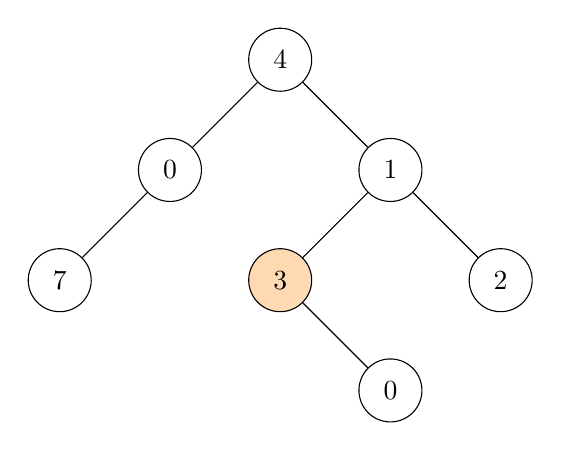
\begin{tikzpicture}[
  level distance=1.4cm,
  sibling distance=2.8cm,
  every node/.style={circle, draw, minimum size=8mm},
  edge from parent/.style={draw,-},
  curr/.style={circle, draw, fill=orange!30}
]
\node {4}
  child { node {0}
    child { node {7} }
    child[missing] {}
  }
  child { node {1}
    child { node[curr] {3}
      child[missing] {}
      child { node {0} }
    }
    child { node {2} }
  };
\end{tikzpicture}

{\small Explore left subtree first (node 3)}
\end{center}

\begin{center}
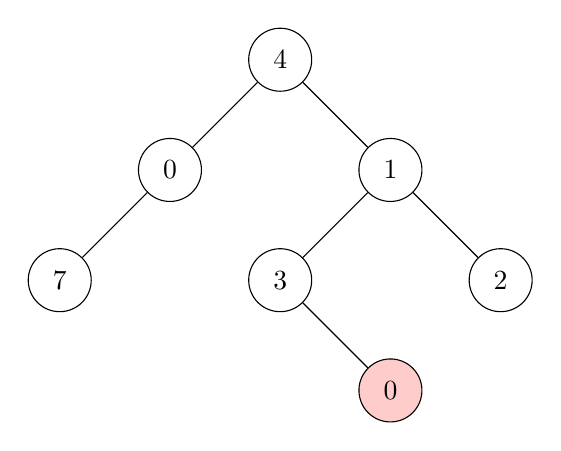
\begin{tikzpicture}[
  level distance=1.4cm,
  sibling distance=2.8cm,
  every node/.style={circle, draw, minimum size=8mm},
  edge from parent/.style={draw,-},
  bad/.style={circle, draw, fill=red!20}
]
\node {4}
  child { node {0}
    child { node {7} }
    child[missing] {}
  }
  child { node {1}
    child { node {3}
      child[missing] {}
      child { node[bad] {0} }
    }
    child { node {2} }
  };
\end{tikzpicture}

{\small Node 3's child is 0 (invalid), return false $\Rightarrow$ backtrack to node 1}
\end{center}

\begin{center}
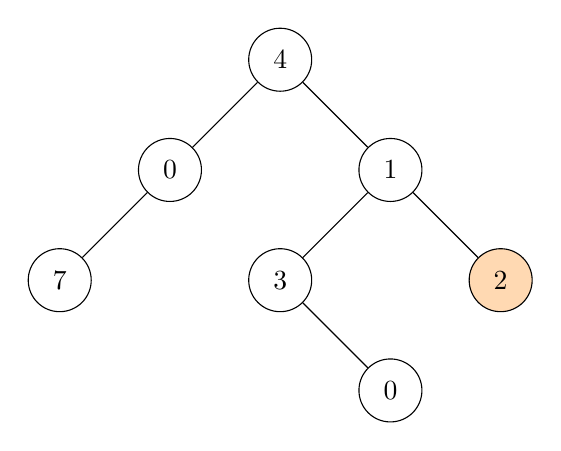
\begin{tikzpicture}[
  level distance=1.4cm,
  sibling distance=2.8cm,
  every node/.style={circle, draw, minimum size=8mm},
  edge from parent/.style={draw,-},
  curr/.style={circle, draw, fill=orange!30}
]
\node {4}
  child { node {0}
    child { node {7} }
    child[missing] {}
  }
  child { node {1}
    child { node {3}
      child[missing] {}
      child { node {0} }
    }
    child { node[curr] {2} }
  };
\end{tikzpicture}

{\small Check node 2 (leaf) — valid path found}
\end{center}

Valid path:
\[
4 \rightarrow 1 \rightarrow 2
\]

% =========================================================
\subsection{Q2: Build the path using backtracking}

Now we must build the path and remove nodes when a branch fails.

\begin{verbatim}
boolean leafPath(TreeNode root, List<Integer> path) {
    if (root == null || root.val == 0) return false;

    path.add(root.val);

    if (root.left == null && root.right == null)
        return true;

    if (leafPath(root.left, path)) return true;
    if (leafPath(root.right, path)) return true;

    path.remove(path.size() - 1);   // backtrack
    return false;
}
\end{verbatim}

\textbf{Step-by-step with live path updates:}

\begin{center}
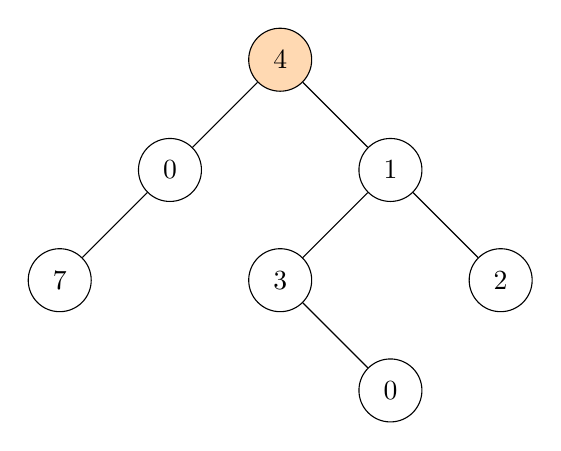
\begin{tikzpicture}[
  level distance=1.4cm,
  sibling distance=2.8cm,
  every node/.style={circle, draw, minimum size=8mm},
  edge from parent/.style={draw,-},
  curr/.style={circle, draw, fill=orange!30}
]
\node[curr] {4}
  child { node {0}
    child { node {7} }
    child[missing] {}
  }
  child { node {1}
    child { node {3}
      child[missing] {}
      child { node {0} }
    }
    child { node {2} }
  };
\end{tikzpicture}

{\small Path = [4]}
\end{center}

\begin{center}
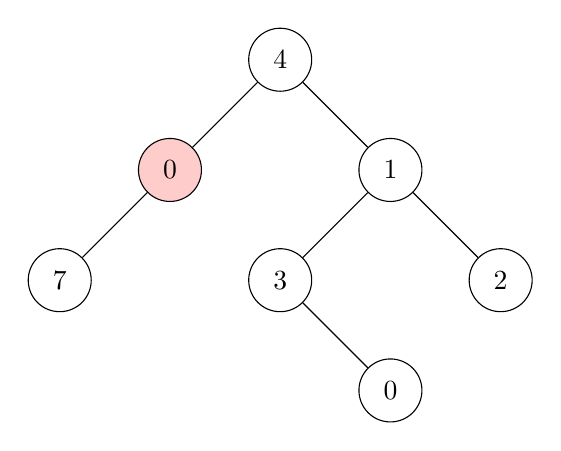
\begin{tikzpicture}[
  level distance=1.4cm,
  sibling distance=2.8cm,
  every node/.style={circle, draw, minimum size=8mm},
  edge from parent/.style={draw,-},
  bad/.style={circle, draw, fill=red!20}
]
\node {4}
  child { node[bad] {0}
    child { node {7} }
    child[missing] {}
  }
  child { node {1}
    child { node {3}
      child[missing] {}
      child { node {0} }
    }
    child { node {2} }
  };
\end{tikzpicture}

{\small Go left: hit 0 (invalid), path unchanged}
\end{center}

\begin{center}
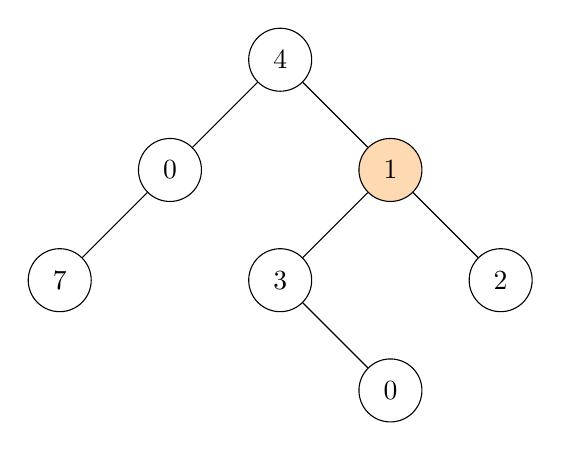
\begin{tikzpicture}[
  level distance=1.4cm,
  sibling distance=2.8cm,
  every node/.style={circle, draw, minimum size=8mm},
  edge from parent/.style={draw,-},
  curr/.style={circle, draw, fill=orange!30}
]
\node {4}
  child { node {0}
    child { node {7} }
    child[missing] {}
  }
  child { node[curr] {1}
    child { node {3}
      child[missing] {}
      child { node {0} }
    }
    child { node {2} }
  };
\end{tikzpicture}

{\small Path = [4, 1]}
\end{center}

\begin{center}
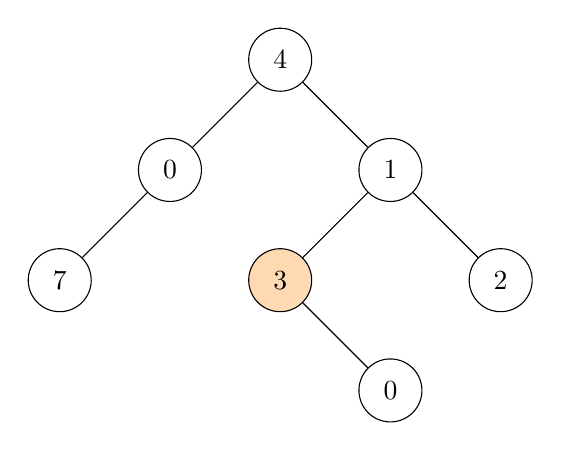
\begin{tikzpicture}[
  level distance=1.4cm,
  sibling distance=2.8cm,
  every node/.style={circle, draw, minimum size=8mm},
  edge from parent/.style={draw,-},
  curr/.style={circle, draw, fill=orange!30}
]
\node {4}
  child { node {0}
    child { node {7} }
    child[missing] {}
  }
  child { node {1}
    child { node[curr] {3}
      child[missing] {}
      child { node {0} }
    }
    child { node {2} }
  };
\end{tikzpicture}

{\small Path = [4, 1, 3]}
\end{center}

\begin{center}
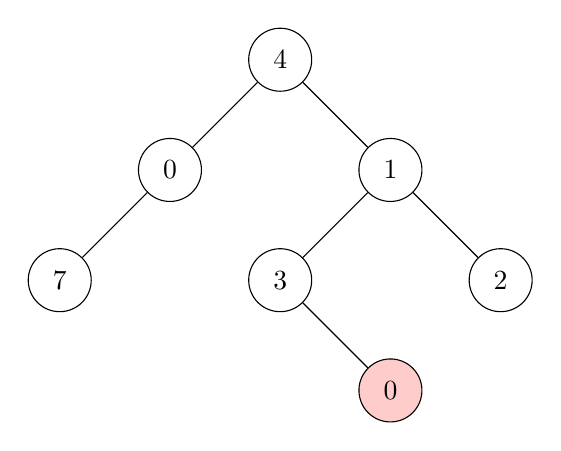
\begin{tikzpicture}[
  level distance=1.4cm,
  sibling distance=2.8cm,
  every node/.style={circle, draw, minimum size=8mm},
  edge from parent/.style={draw,-},
  bad/.style={circle, draw, fill=red!20}
]
\node {4}
  child { node {0}
    child { node {7} }
    child[missing] {}
  }
  child { node {1}
    child { node {3}
      child[missing] {}
      child { node[bad] {0} }
    }
    child { node {2} }
  };
\end{tikzpicture}

{\small From node 3, child is 0 (invalid) $\Rightarrow$ backtrack, pop 3}
\end{center}

\begin{center}
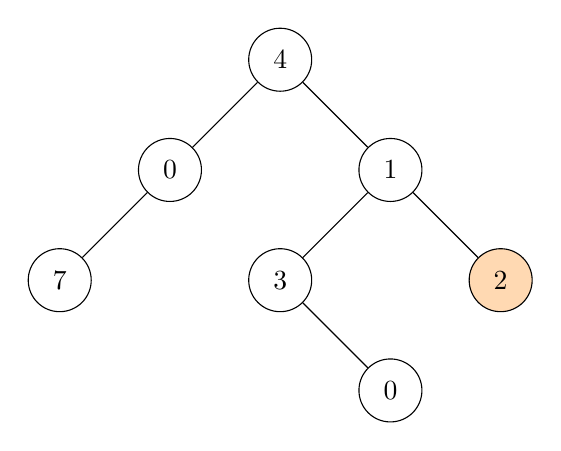
\begin{tikzpicture}[
  level distance=1.4cm,
  sibling distance=2.8cm,
  every node/.style={circle, draw, minimum size=8mm},
  edge from parent/.style={draw,-},
  curr/.style={circle, draw, fill=orange!30}
]
\node {4}
  child { node {0}
    child { node {7} }
    child[missing] {}
  }
  child { node {1}
    child { node {3}
      child[missing] {}
      child { node {0} }
    }
    child { node[curr] {2} }
  };
\end{tikzpicture}

{\small Path = [4, 1, 2] (leaf)}
\end{center}

Final path:
\[
[4, 1, 2]
\]

\subsection{Time and Space Complexity}
\begin{itemize}
  \item \textbf{Time:} $O(n)$ — may visit all nodes
  \item \textbf{Space:} $O(h)$ — recursion depth and path length
\end{itemize}